\documentclass{beamer}
\usepackage{subfig}
\usepackage{amsmath}
\usepackage{bm}


\DeclareMathOperator*{\argmax}{arg\,max}
\DeclareMathOperator*{\argmin}{arg\,min}

\setbeamertemplate{footline}[frame number]
\title{Regression and Gradient Descent}
\author{Prof. Alessandro Lucantonio}
\institute{Aarhus University}
\date{24/10/2023}

\setbeamertemplate{navigation symbols}{}


\begin{document}
	
	\frame{\titlepage}
	
	\section{Linear regression with one variable}

	\begin{frame}
		\frametitle{Weight-Height dataset}
		
		Task: build a model that predicts the height given the weight. 
		
		\begin{figure}
			\centering
			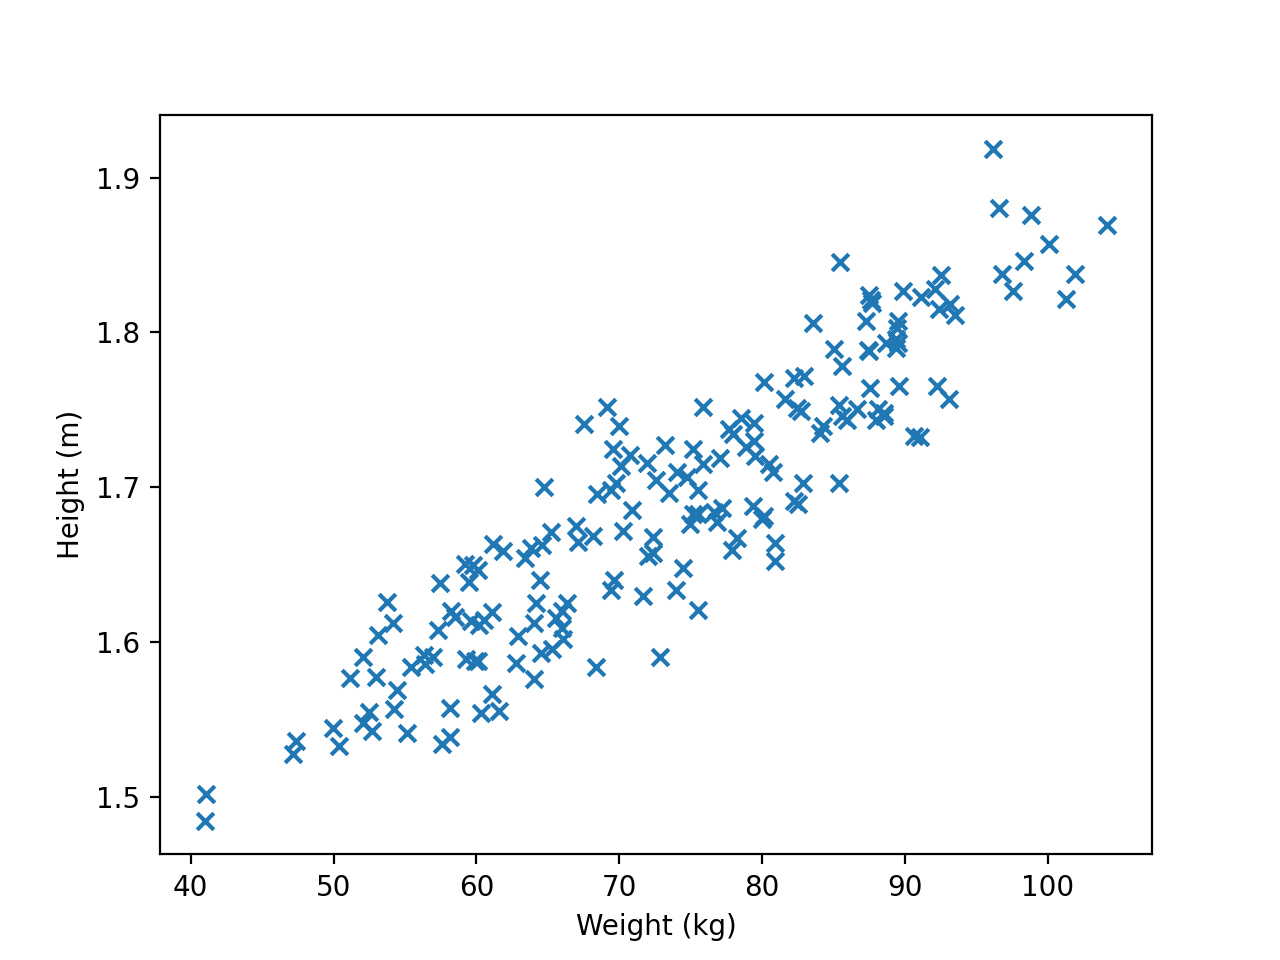
\includegraphics[scale=0.5]{images/linear_regression_data}
			\caption{Plot of the dataset}
		\end{figure}
	\end{frame}

	\begin{frame}
		\frametitle{A solution - Linear Regression model}
		Remarks:
		\begin{itemize}
			\item Regression problem (continuous output).
			\item Data with different orders of magnitude.
		\end{itemize}
		A possible solution to this problem is a linear model (red line in the figure below). This learning algorithm is called \textbf{Linear Regression} (LR).
		\vspace{-5mm}
		\begin{figure}
			\centering
			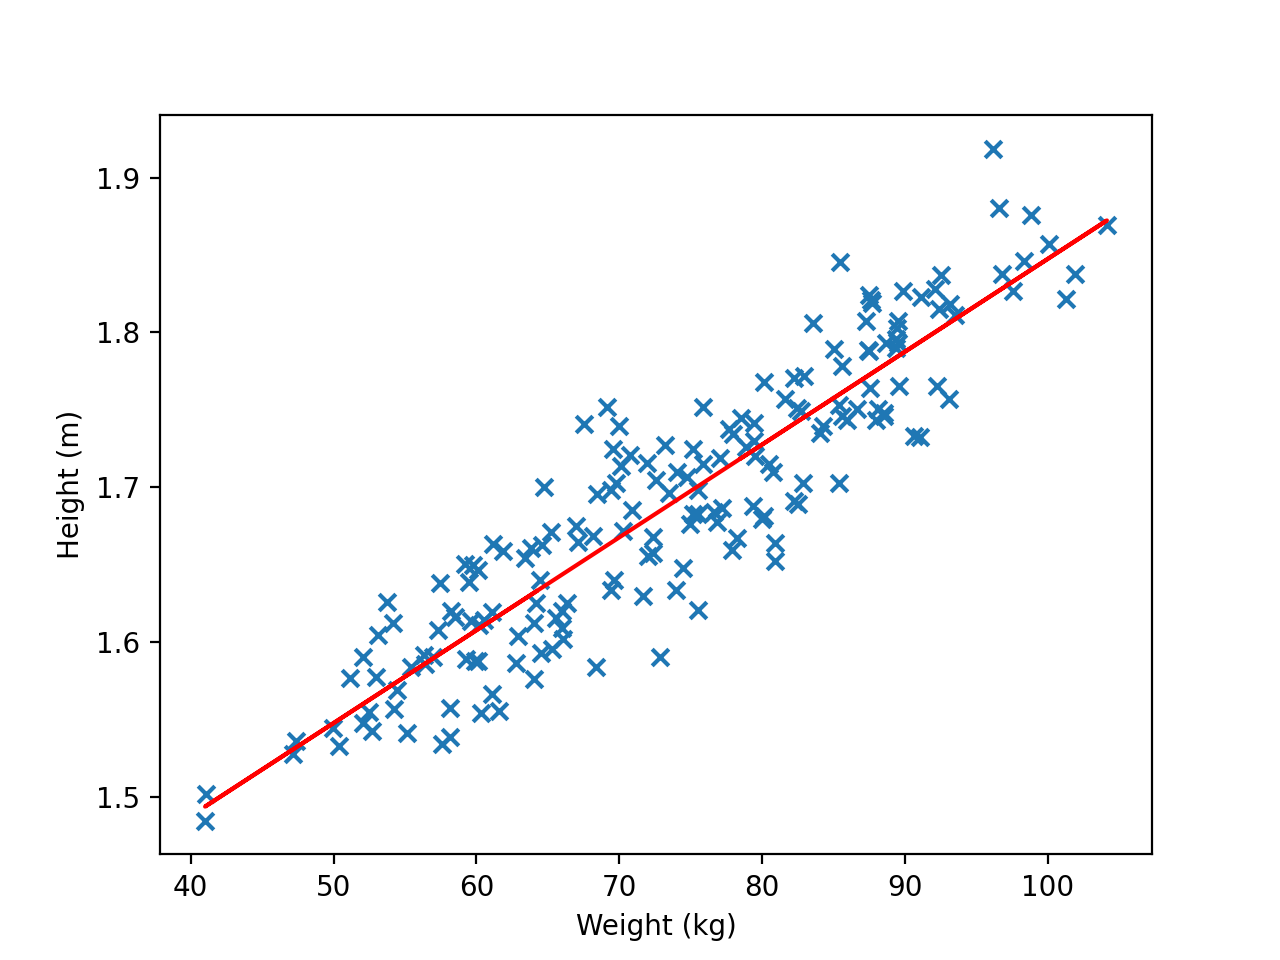
\includegraphics[scale=0.4]{images/linear_regression_fit}
			\caption{Linear regression model.}
		\end{figure}
	\end{frame}

	\begin{frame}
		\frametitle{Linear Regression: main ingredients}
		Notation:
		\begin{itemize}
			\item $x^{(i)}$: a data sample (weight of the $i$-th person).
			\item $y^{(i)}$: the target corresponding to $x^{(i)}$ (height).
			\item $N$: number of samples.
		\end{itemize}
	
		\vspace{5 mm}
		
		\textbf{Model/hypothesis}: 
		\begin{align*}
			h_{\bm{w}}(x^{(i)}) = w_1x^{(i)} + w_0
		\end{align*}
		where $\bm{w} = [w_0, w_1]^T$ is the vector of parameters to be learned.
		
		\vspace{5 mm}
		
		The set $\mathcal{H}:= \{h_{\bm{w}}| \bm{w} \in \mathbb{R}^2\}$ is called \textbf{hypothesis space}.
		
		\vspace{5 mm}
		
		How to learn $\bm{w}$ from data?
		
	\end{frame}

	\begin{frame}
		\frametitle{Performance measure: Mean Squared Error (MSE)}
		To evaluate how good is the prediction we compute the \textbf{Mean Squared Error} (MSE) is:
		$$E({\bm{w}}) := \frac{1}{N} \sum_{i=1}^{N} (h_{\bm{w}}(x^{(i)}) - y^{(i)})^2.$$
		
		To find the ``best" set of parameters, we minimize the MSE:
		
		$$\bm{w} \in \argmin_{\tilde{\bm{w}} \in \mathbb{R}^2} E(\tilde{\bm{w}}).$$
		
	\end{frame}

%	\begin{frame}
%		\frametitle{MSE - Visualization}
%		\begin{figure}
%			\centering
%			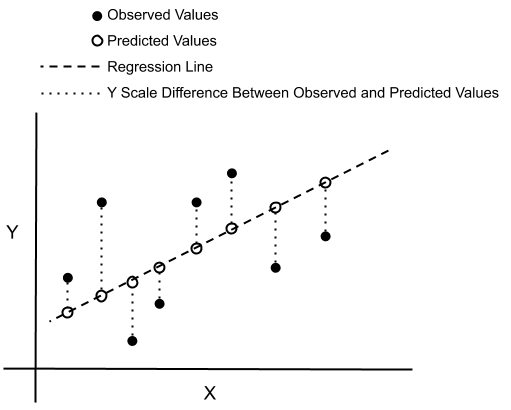
\includegraphics[scale=0.5]{images/mse}
%		\end{figure}
%	\end{frame}

	\begin{frame}
		\frametitle{Multiple-feature Linear Regression}
		
		\begin{itemize}
			\item Dataset: $\bm{x}^{(i)} \in \mathbb{R}^n, y^{(i)} \in \mathbb{R}$, where
			$x^{(i)}_j$ is the $j$-th feature of the $i$-th sample and $n$ is the number of features.
			\item Hypothesis: 
			\begin{align*}
				h_{\bm{w}}(\bm{x}^{(i)}) &= w_{n}x^{(i)}_n + w_{n-1}x^{(i)}_{n-1} + \dots + w_1 x^{(i)}_1 + w_0\\
				&= \sum_{i=0}^n w_i \tilde{x}^{(i)}_i = \bm{w}^T \tilde{\bm{x}}^{(i)},
			\end{align*}
			where $\bm{w} = [w_0, \dots, w_n]^T$ and $\tilde{\bm{x}}^{(i)} = [1, x^{(i)}_1, \dots, x^{(i)}_n]^T$.
		\end{itemize}
		
	\end{frame}

	\begin{frame}
		\frametitle{Multiple-feature Linear Regression - MSE}
		\textsl{MSE}:
		\begin{align*}
			E(\bm{w}) &= \frac{1}{N} \sum_{i=1}^{N} (h_{\bm{w}}(\bm{x}^{(i)}) - y^{(i)})^2\\
			&= \frac{1}{N} (\mathsf{X} \bm{w} - \bm{y})^T (\mathsf{X}\bm{w} - \bm{y})\\
			&= \frac{1}{N} ||\mathsf{X}\bm{w} - \bm{y}||^2
		\end{align*}
		where
		\begin{equation*}
			\mathsf{X} = \begin{bmatrix}
				(\tilde{\bm{x}}^{(1)})^T\\
				\vdots\\
				(\tilde{\bm{x}}^{(N)})^T
			\end{bmatrix} \quad \bm{y} = \begin{bmatrix}
			y^{(1)} \\
			\vdots\\
			y^{(N)}
		\end{bmatrix}.
		\end{equation*}
	Notice that $\mathsf{X} \in \mathbb{R}^{N \times (n+1)}$ and $\bm{y} \in \mathbb{R}^N$.
	\end{frame}

	\begin{frame}
		\frametitle{Coefficient of determination}
		Idea: $\mathsf{X}$ and $\bm{y}$ can be thought as two random variables.
		
		\vspace{5mm}
		
		Let $\bm{\epsilon} := \bm{y} - \mathsf{X}\bm{w}$ the vector of the residuals and $\sigma_{\bm{y}}:= \sqrt{\text{Var}(\bm{y})}$ the standard deviation of the targets.  The quantity
		\begin{equation*}
			R^2 := 1 - \frac{||\bm{\epsilon}||^2}{\sigma_{\bm{y}}^2}
		\end{equation*}
		is called the \textsl{coefficient of determination}.
		
		\vspace{5mm}
		
		Best case scenario: $\sigma_{\bm{\epsilon}} = 0$, hence $R^2 = 1$.
		
	\end{frame}

	\begin{frame}
		\frametitle{Finding the minimum: Gradient Descent}
		How to find $\bm{w} \in \argmin_{\tilde{\bm{w}} \in \mathbb{R}^2} E(\tilde{\bm{w}})$?
		
		\vspace{5mm}
		
		Main idea: geometrically, the gradient of a scalar function represents the direction of maximum slope. Hence, following the direction opposite to the gradient allows to decrease the value of the function, \textit{i.e.}
		\begin{equation*}
			E(\bm{w}^{j+1}) \leq E(\bm{w}^j) 
		\end{equation*}
		
		\vspace{5mm}
		
		Formally:
		\begin{itemize}
			\item Start with an initial guess $\bm{w}^0$.
			\item For $j \geq 0$, update $\bm{w}^{j+1} := \bm{w}^{j} + \bm{d}^j$, where $\bm{d}^j$ is such that
			$$\bm{d}^j = - \alpha \nabla E(\bm{w}^j)$$
			where $\alpha>0$ is the \textbf{learning rate}.
		\end{itemize}
	
	\end{frame}

	\begin{frame}
		\frametitle{Gradient Descent - 3D visualization}
		\begin{figure}
			\centering
			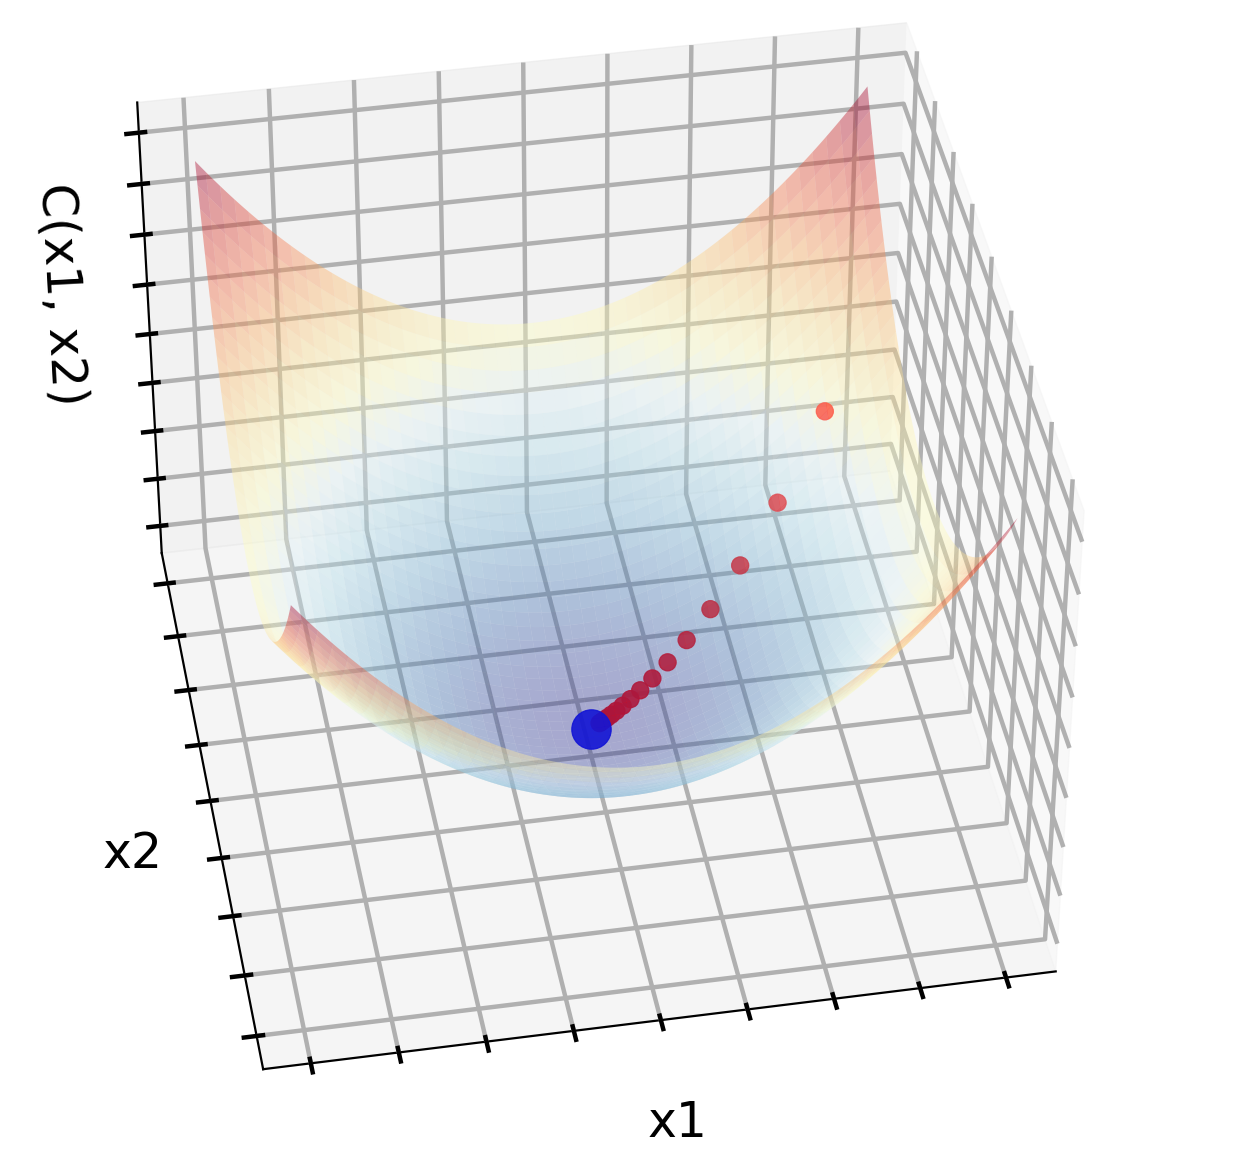
\includegraphics[scale=0.4]{images/gradient_descent_3D}
			\caption{n blue the global minimum, in red the iteration points.}
		\end{figure}
	\end{frame}

	\begin{frame}
		\frametitle{Gradient Descent: Effect of the learning rate/1}
		\begin{figure}
			\centering
			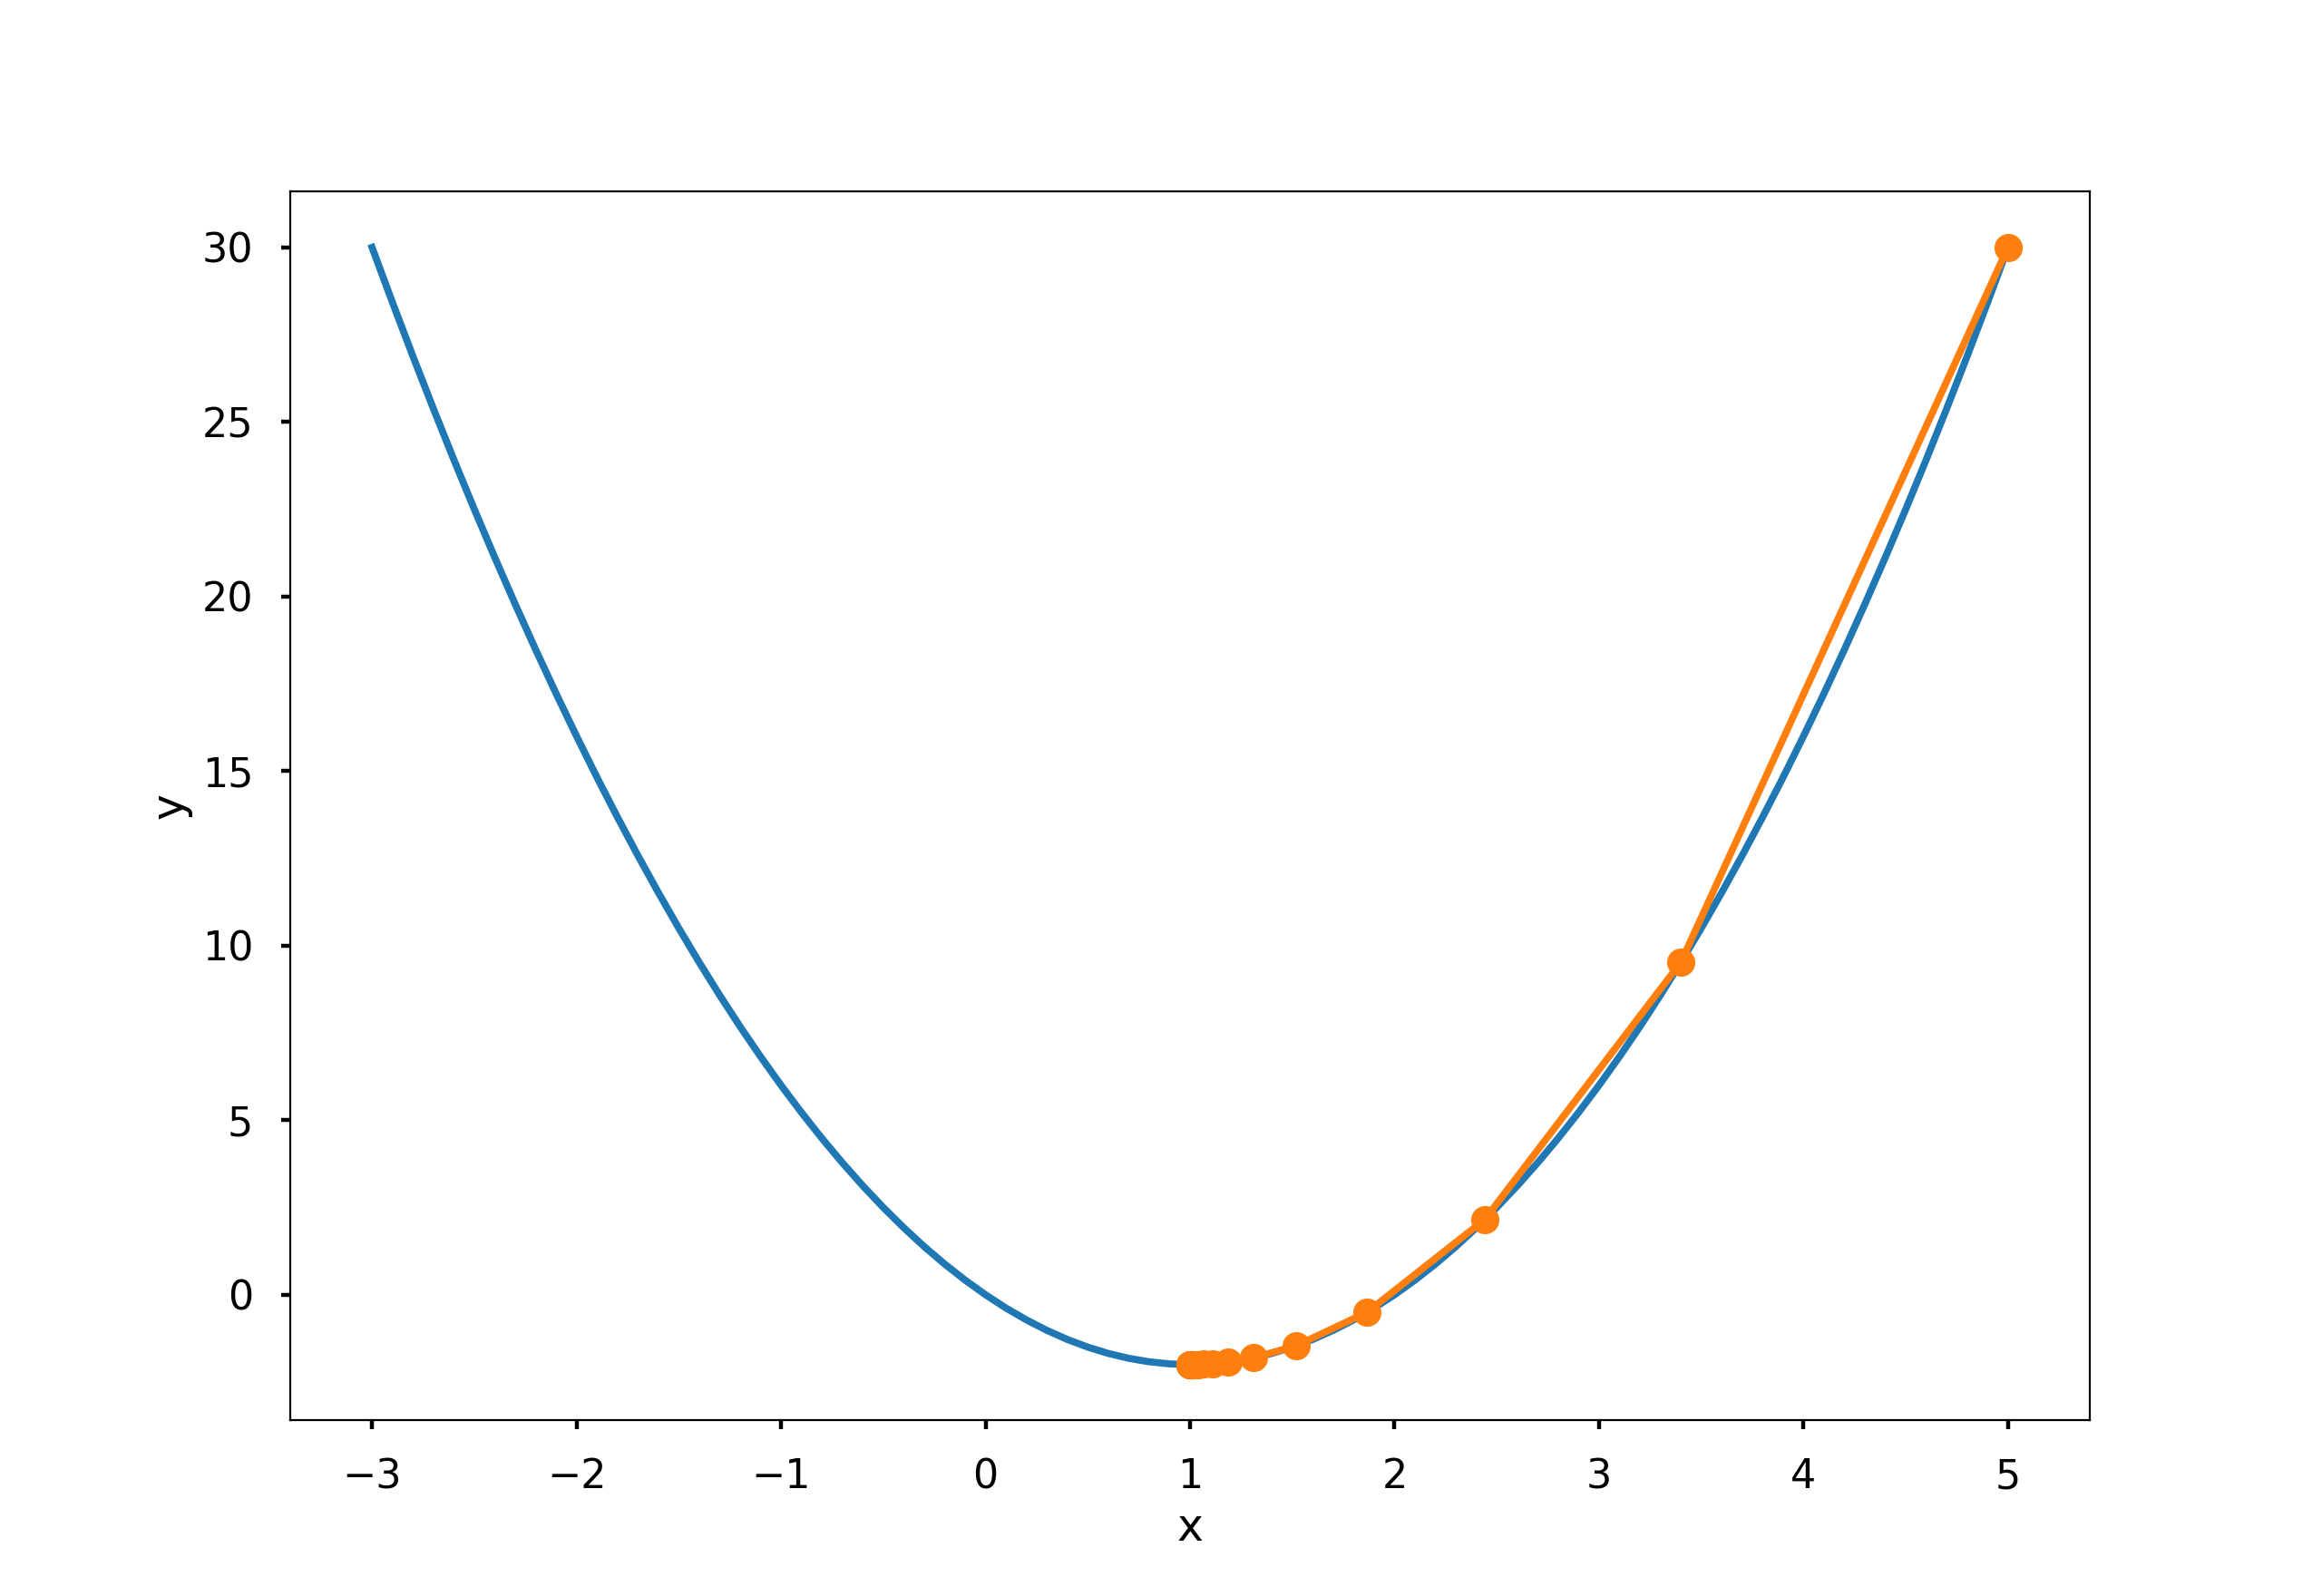
\includegraphics[scale=0.3]{images/gradient_descent_1}
			\caption{Learning rate = 0.1}
		\end{figure}
	\end{frame}

	\begin{frame}
		\frametitle{Gradient Descent: Effect of the learning rate/2}
		\begin{figure}
			\centering
			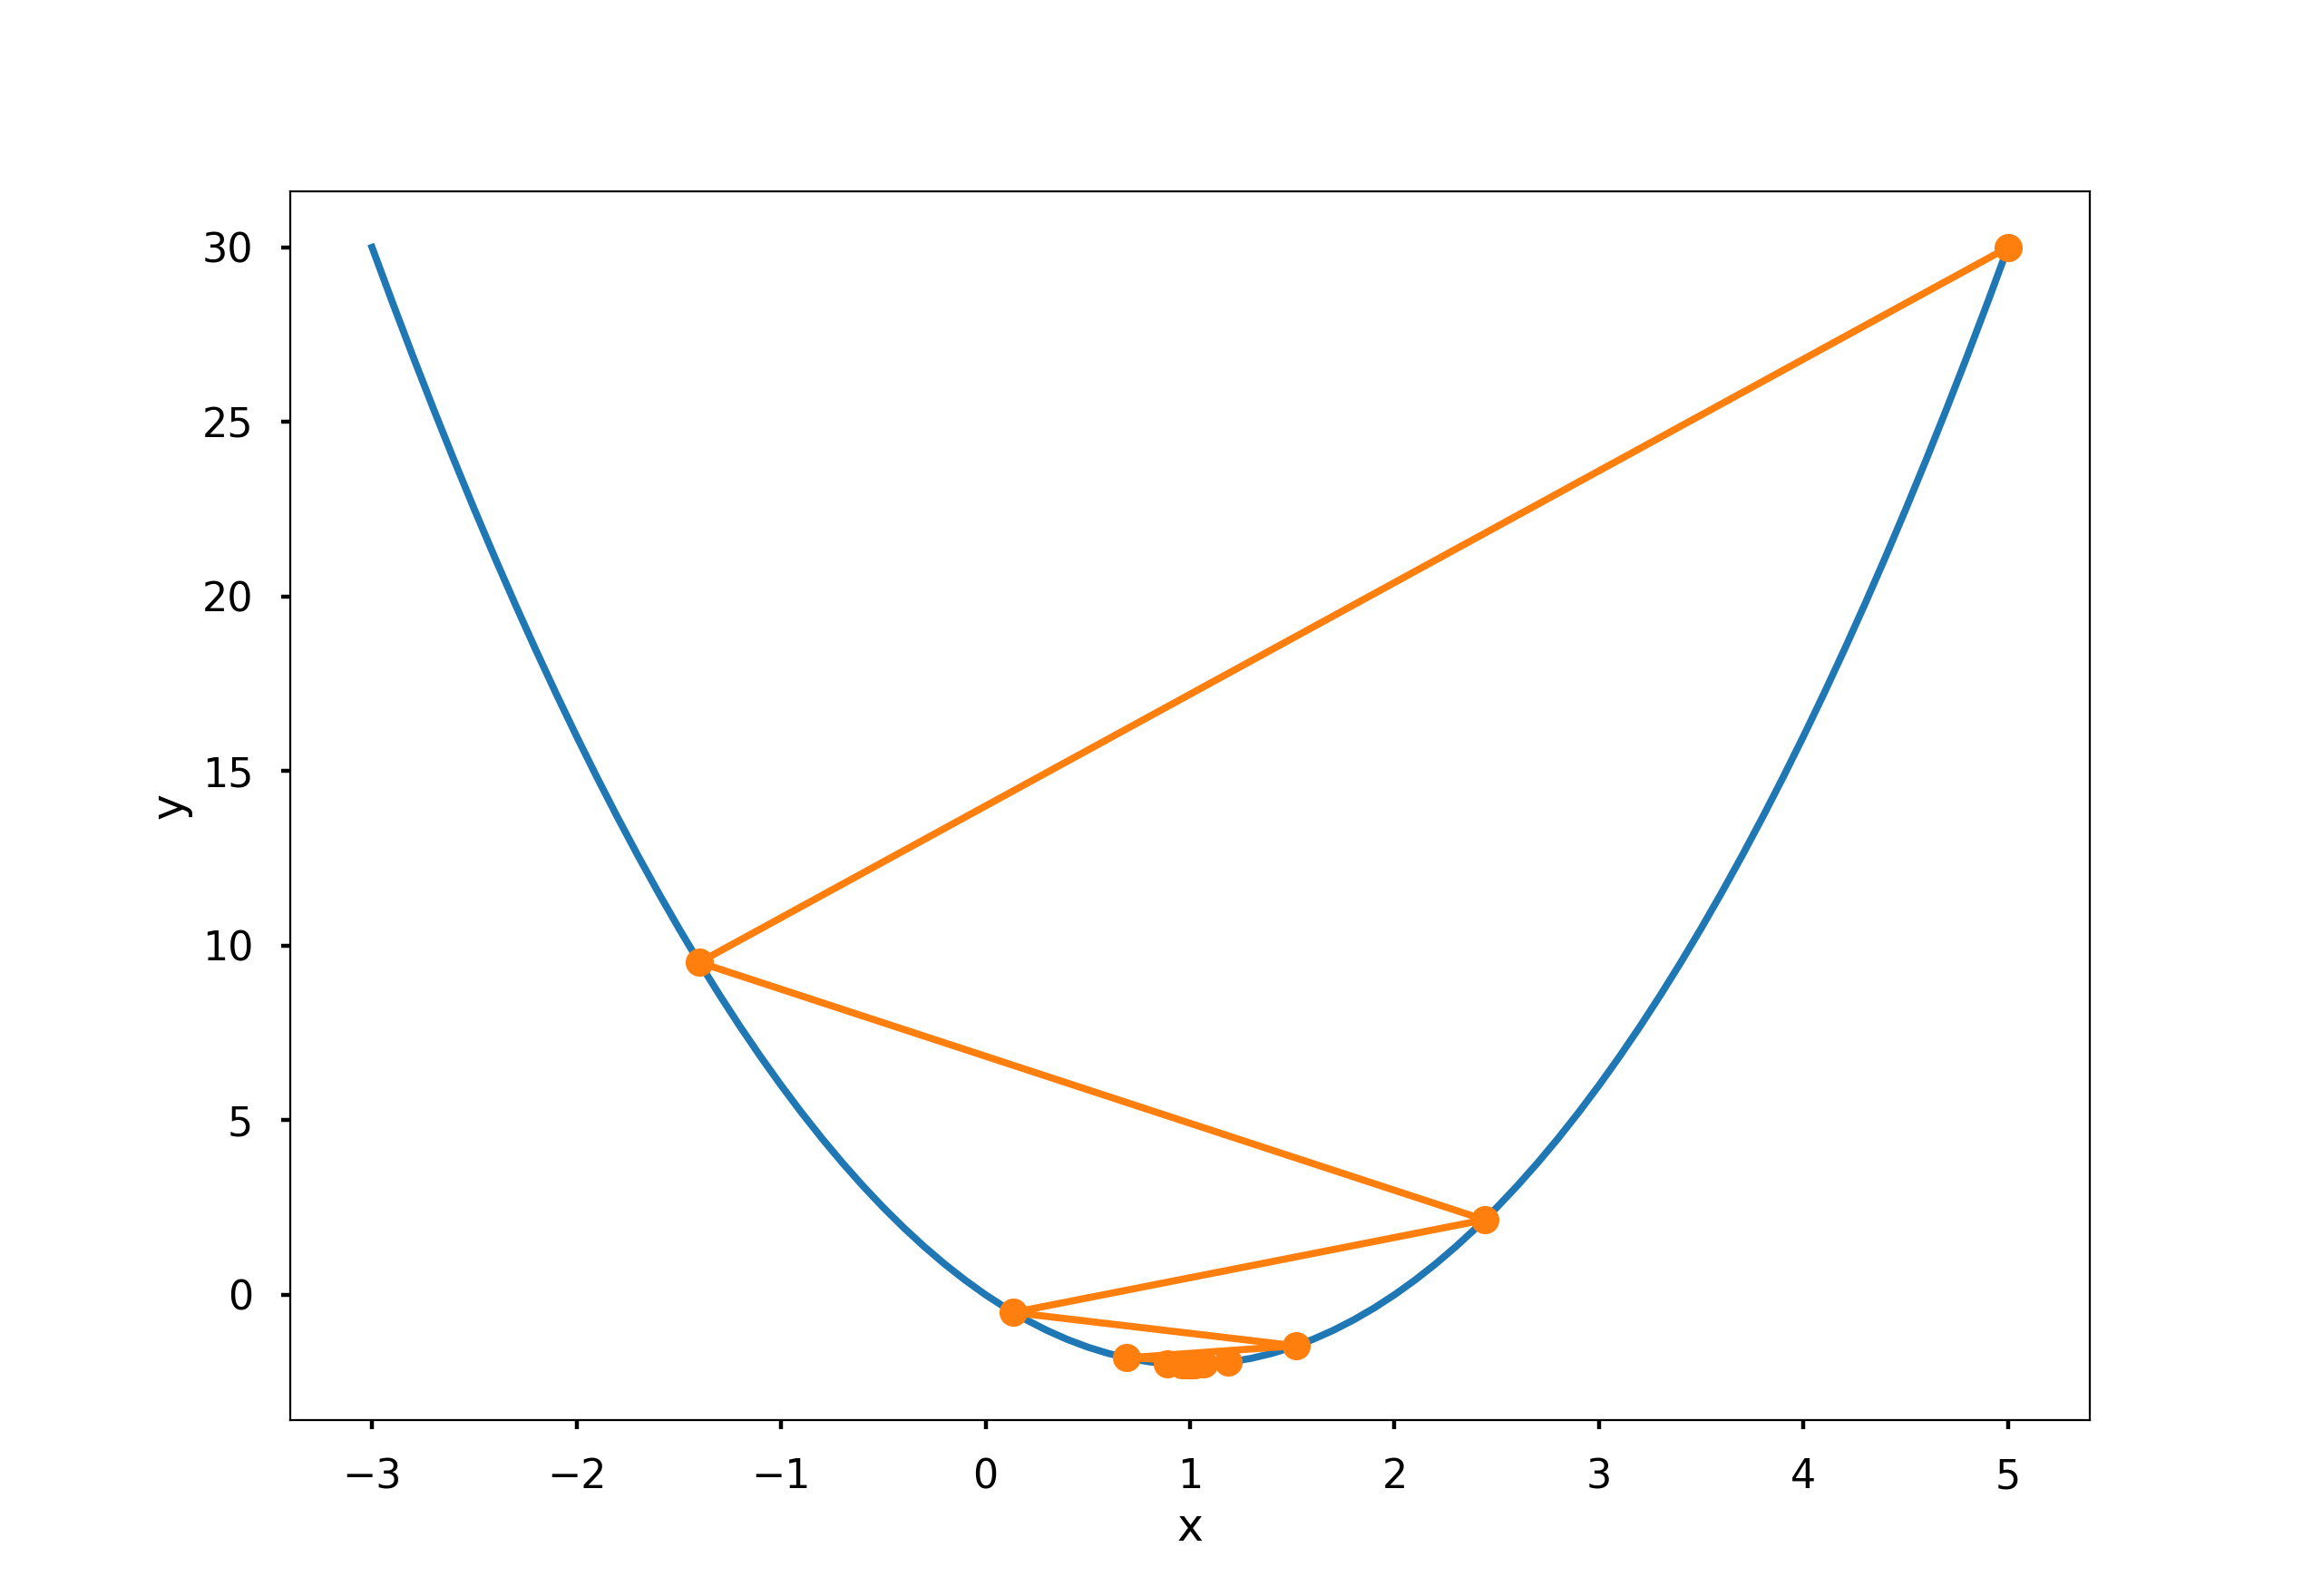
\includegraphics[scale=0.3]{images/gradient_descent_2}
			\caption{Learning rate = 0.4}
		\end{figure}
	\end{frame}

	\begin{frame}
		\frametitle{Gradient Descent: Effect of the learning rate/3}
		\begin{figure}
			\centering
			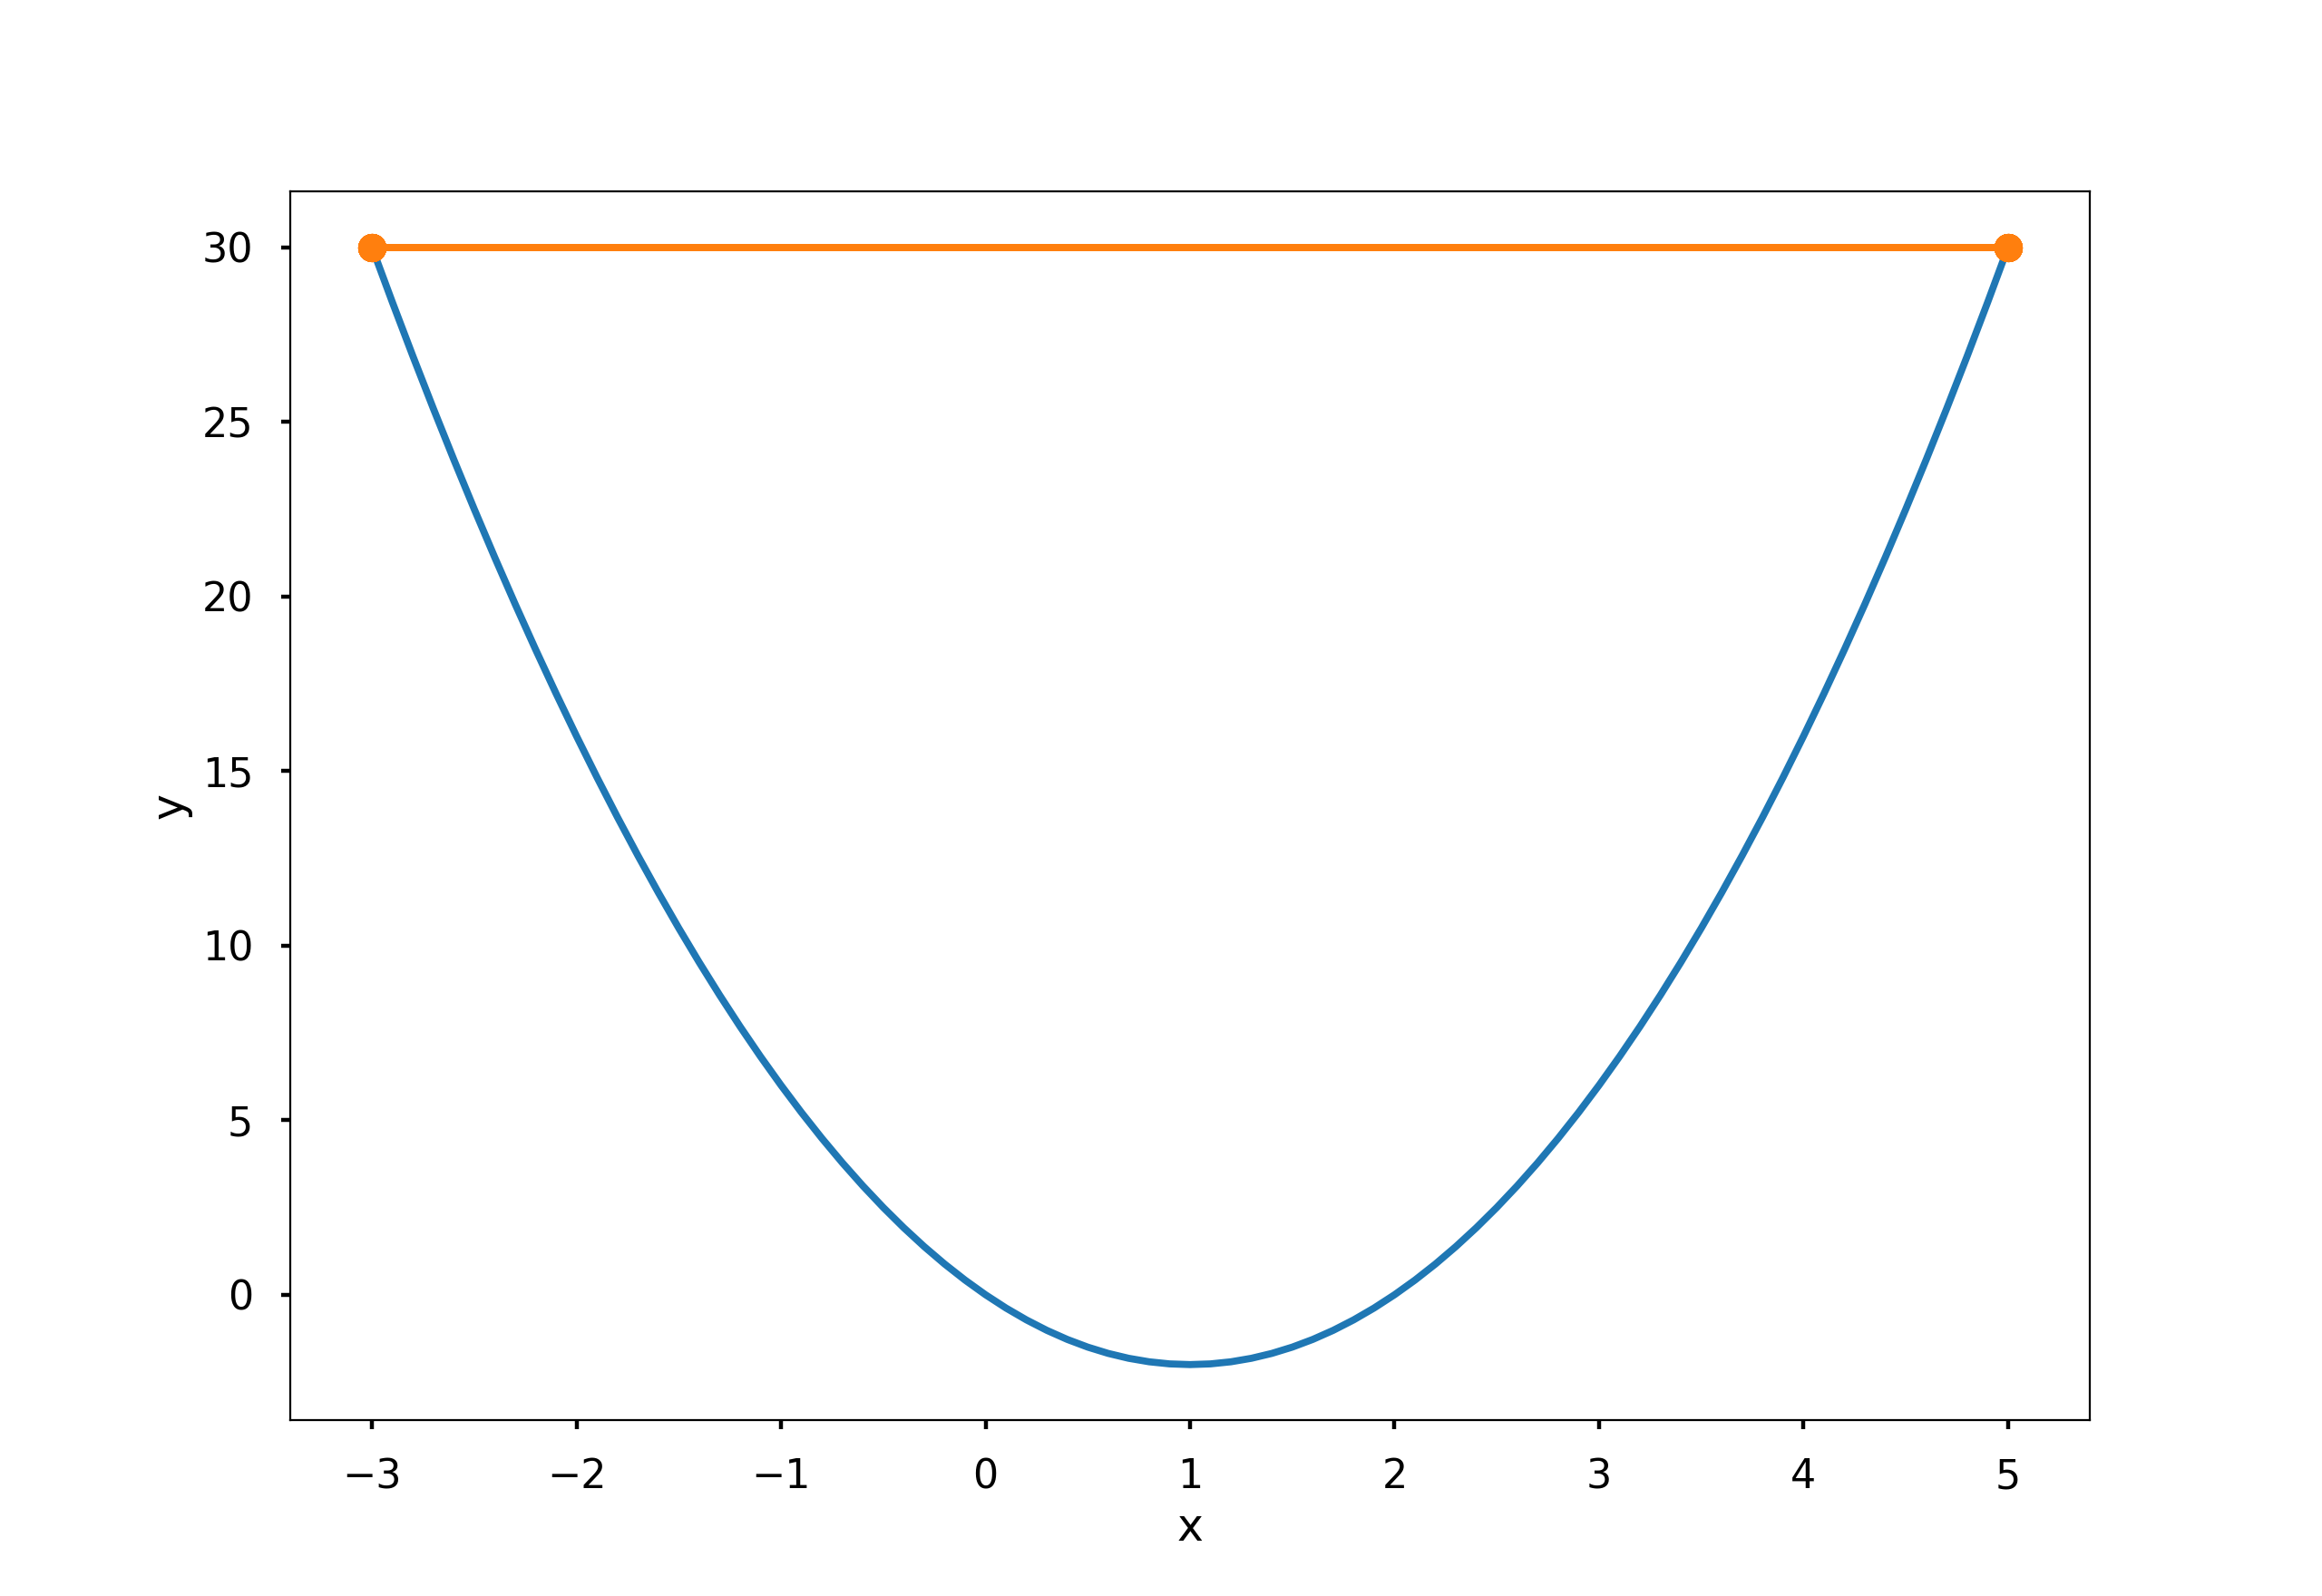
\includegraphics[scale=0.3]{images/gradient_descent_3}
			\caption{Learning rate = 0.5}
		\end{figure}
	\end{frame}

	\begin{frame}
		\frametitle{Batch GD, SGD and Mini-Batch GD - Intuition}
		Notation: $E(\bm{w}) = 1/N \sum_{i=1}^N E_i(\bm{w})$
		
		The classical gradient descent update rule, \textit{i.e.} update the weights computing the gradient of the entire cost (error) function $E(\bm{w})$, is called \textbf{batch version}. However, for large number of samples ($N$) computing $\nabla E(\bm{w})$ is very time consuming.
		
		\vspace{5mm}
		
		To speed-up the update rule we approximate $\nabla E(\bm{w})$ with $\nabla E_i(\bm{w})$. This is the idea behind the so-called \textbf{Stochastic Gradient Descent} (SGD) or \textbf{online version}.
		
		\vspace{5mm}
		
		A trade-off between batch GD and SGD is called the \textbf{mini-batch} GD.
	\end{frame}

	\begin{frame}
		\frametitle{Batch GD, SGD and Mini-Batch GD - Algorithms}
		
		
		\textbf{Batch GD}
		\begin{itemize}
			\item Start with an initial guess $\bm{w}^0$.
			\item For $j \geq 0$, update $\bm{w}^{j+1} := \bm{w}^{j} - \alpha \nabla E(\bm{w}^j)$.
		\end{itemize}
		
		\textbf{SGD} (online)
		\begin{itemize}
			\item Start with an initial guess $\bm{w}^0$.
			\item For each epoch $j \geq 0$:
			\begin{itemize}
				\item draw a random sample $i$ from the dataset;
				\item for each $1\leq i \leq N$ update $\bm{w} = \bm{w} - \alpha \nabla E_i(\bm{w})$.
			\end{itemize}
		\end{itemize}
	
		\textbf{Mini-Batch GD}
		\begin{itemize}
			\item Fix an integer $1 \leq \text{mb} \leq N$ (mini-batch size).
			\item Start with an initial guess $\bm{w}^0$.
			\item For each epoch $j \geq 0$:
			\begin{itemize}
				\item draw a random batch from the dataset;
				\item for each $0 \leq i < \frac{N}{\text{mb}}$ update
				\begin{equation*}
					\bm{w} := \bm{w} - \alpha \nabla \sum_{k=i\cdot\text{mb} + 1}^{(i+1)\cdot\text{mb}}E_k(\bm{w}).
				\end{equation*}
			\end{itemize} 
		\end{itemize}
		
	\end{frame}

	\begin{frame}
		\frametitle{Tips and Tricks - How to choose?}
		\begin{itemize}
			\item Batch: usually more stable and provide a more accurate estimation of the gradient, but slow.
			\item SGD: fast, stochastic approximation of the gradient implies possible instability (zig-zag effect)
			\item Mini-Batch GD: a trade-off between Batch GD and SGD (parallelism available).
		\end{itemize}
	%In practice, through SGD and Mini-Batch GD we may not even reach the minimum, but it is enough to get close to it.
		\begin{figure}
			\centering
			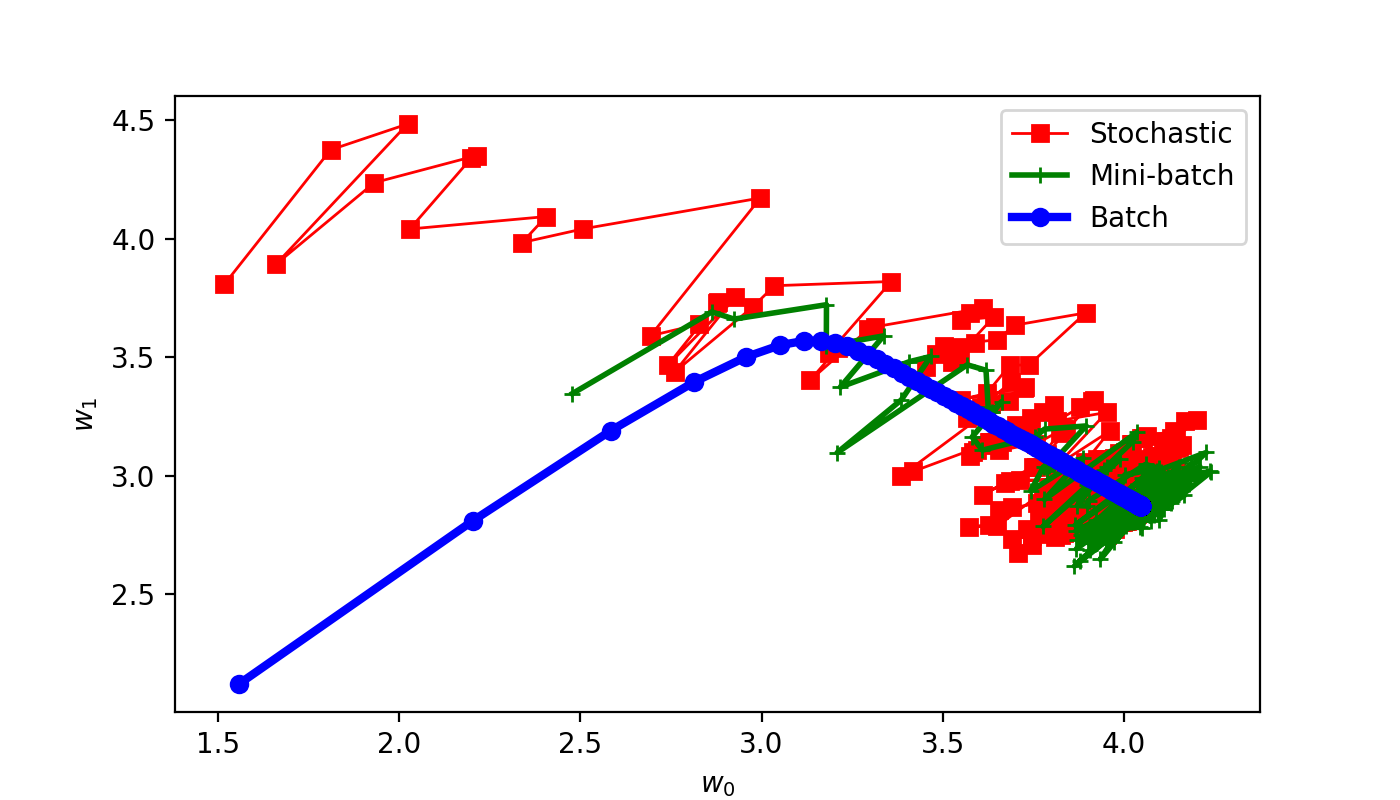
\includegraphics[scale=0.42]{images/gd_mb_sgd}
			\caption{Batch GD vs SGD vs Mini-Batch GD}
		\end{figure}
	
	\end{frame}

	\begin{frame}
		\frametitle{Normal Equation for LR and Gradient Descent}
		We have $E(\bm{w}) = \frac{1}{N} ||\mathsf{X}\bm{w} - \bm{y}||^2$, hence
		\begin{equation*}
			\nabla E(\bm{w}) = \frac{1}{N} \nabla (||\mathsf{X}\bm{w} - \bm{y}||^2) = \frac{2}{N}\mathsf{X}^T(\mathsf{X}\bm{w} - \bm{y})
		\end{equation*}
	
	\begin{itemize}
		\item 	Normal equation ($\textcolor{red}{\iff}$ holds if $\mathsf{X}^T\mathsf{X}$ is invertible):
		\begin{align*}
			\nabla E(\bm{w}) = 0 &\iff \frac{2}{N}\mathsf{X}^T(\mathsf{X}\bm{w} - \bm{y}) = 0\\ 
			&\iff \mathsf{X}^T\mathsf{X}\bm{w} = \mathsf{X}^T\bm{y}\\
			& \textcolor{red}{\iff} \bm{w} = (\mathsf{X}^T\mathsf{X})^{-1}\mathsf{X}^T\bm{y}
		\end{align*}
		\item Gradient descent main iteration for LR:
		\begin{equation*}
			\bm{w}^{j+1} := \bm{w}^{j} - \frac{2\alpha}{N}\mathsf{X}^T(\mathsf{X}\bm{w}^j - \bm{y})
		\end{equation*}
	\end{itemize}

	\end{frame}

	\begin{frame}
		\frametitle{Tips and Tricks - Invertibility of $\mathsf{X}^T\mathsf{X}$}
		
		Invertibility of $\mathsf{X}^T\mathsf{X} \iff$ columns of $X$ linearly independent.
		
		\vspace{5mm}
		
		What if $\mathsf{X}^T\mathsf{X}$ is not invertible?
		
		\vspace{5mm}
		
		If two columns are linearly dependent, then those features are correlated (\textbf{redundant}).
		
		\vspace{5mm}
		
		Solution: discard one of those features.
	\end{frame}

	\begin{frame}
		\frametitle{Normal Equation vs Gradient Descent}
		Normal equation:
		\begin{itemize}
			\item No hyperparameters (explicit solution).
			\item No iterations.
			\item $\mathcal{O}(N^3)$, since this is the cost to invert a dense matrix. In particular, it is slow when $N$ is large.
		\end{itemize}
	
		\vspace{5mm}
	
		Gradient Descent:
		\begin{itemize}
			\item Need to choose the learning rate $\alpha$.
			\item Needs many iterations.
			\item $\mathcal{O}(N^2)$, hence faster when $N$ is large.
		\end{itemize}
	\end{frame}


	\begin{frame}
		\frametitle{Tips and Tricks - Standardization}
		General (not only for LR): features must have similar magnitudes!
		\begin{itemize}
			\item Speed up the convergence of gradient descent.
			\item Try to have (on average) $-1 \leq \bm{x}^{(i)} \leq 1$.
		\end{itemize}
		Common techniques:
		\begin{itemize}
			\item \textbf{Feature scaling}. Compute the feature max $\bm{M} := [\max_i x^{(i)}_j]$ and the feature min $\bm{m} := [\min_i x^{(i)}_j]$ vectors. Then normalize features as follows
			\begin{equation*}
				\bm{x}_{\text{norm}}^i = \frac{\bm{x}^{(i)} - \bm{m}}{\bm{M} - \bm{m}}
			\end{equation*} 
			\item \textbf{Mean normalization}. Compute the feature mean $\bm{\mu}$ $(\mu_j := \mathbb{E}[[x^{(i)}_j]_i])$ and the feature standard deviation $\bm{\sigma}$ $(\sigma_j := \sqrt{\text{Var}[[x^{(i)}_j]_i]})$. Then normalize features as follows
			\begin{equation*}
				\bm{x}_{\text{norm}}^{(i)} = \frac{\bm{x}^{(i)} -\bm{\mu}}{\bm{\sigma}} 
			\end{equation*}
		\end{itemize}
	\end{frame}

	\begin{frame}
		\frametitle{Tips and Tricks - Standardization}
		\begin{figure}
			\centering
			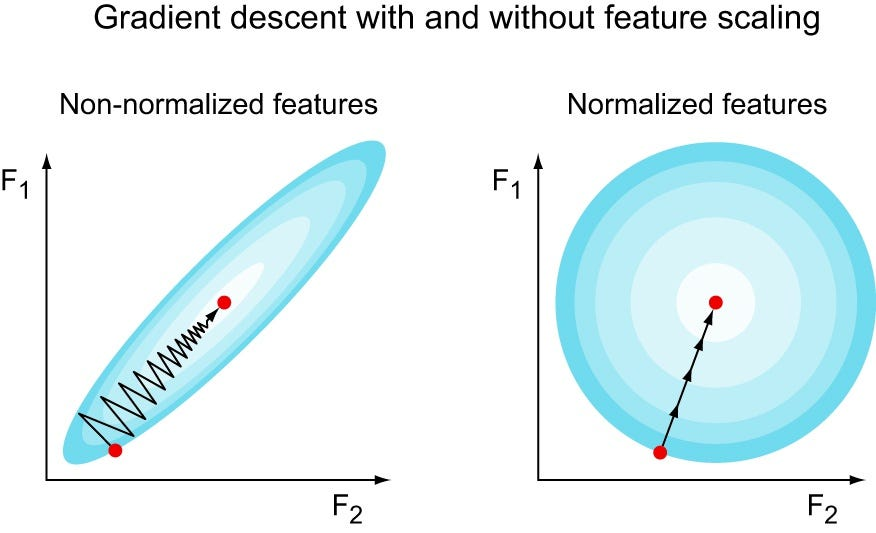
\includegraphics[scale=0.35]{images/feature-scaling}
		\end{figure}

		
	\end{frame}



	\begin{frame}
		\frametitle{Polynomial regression (PR)}
		PR corresponds to polynomial hypothesis, i.e. of the form
		\begin{equation*}
			h_{\bm{w}}(\bm{x}) = \sum_{j=0}^n w_j x^j_j.
		\end{equation*}
		
		\vspace{5mm}
		More in general: linear basis expansion (LBE)
		\begin{equation*}
			h_{\bm{w}}(\bm{x}) = \sum_{j=0}^n w_j \phi_j(\bm{x}),
		\end{equation*}
		where $\phi_j: \mathbb{R}^n \rightarrow \mathbb{R}$.
	\end{frame}


\end{document}